% NOTES 
% Wie ich den sprinback gemssen habe 

\chapter{Build}

\section{Dataset generation}
For the dataset generation, bending experiments were performed on metal sheets with different thicknesses.
% material
The material used is cold rolled steel sheets of the norm DIN EN 10130. The thicknesses used were 0.5mm, 1mmm and 2mm.
The material was used because it is commonly used in bending processes and its high availability. In previous tests, it was observed, that the spring back are well observable with this material.
Using this material, 200 single bending pieces of the dimension 20×100 mm have been cut.
Each piece was bend one time using a \textit{Zwick} three-point-bending machine.

Python script where developed to covert the output data format from the machine to CSV files.
The following describes the experimental setup used for the experiments performed.

\subsection{Experimental setup}
The setup consists of a three-point-bending machine with a punch and a die with no bottom. The machine used is the \textit{Zwick MX 25A} material testing machine. 
The machine is equipped with a load cell and a displacement sensor. The load cell is used to measure the force applied to the sheet and the displacement sensor is used to measure the displacement of the punch.
The machine is controlled by a computer and a software called \textit{ZwickRoell TestXpert}. The software is used to control the machine and to save the output data.

The experimental setup and its parameters are shown in Figure~\ref{fig:setup} where $V$ is the die opening, $y_p$ is the punch penetration which is the distance the punch is moved into the sheet. 
The paramter $t$ is the sheet thickness,  $\alpha$ is the sheet corresponding bending angle. Parameter $r_p$ is the punch radius which is the radius of the tip of the punch and $r_m$ is the die radius.



\begin{figure}[H]
    \centering
    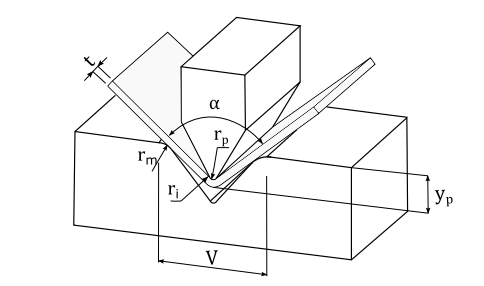
\includegraphics[width=0.6\textwidth]{setup}
    \caption{Experimental setup: sheet bending angle ($\alpha$), sheet thickness ($t$), punch penetration ($y_p$), die opening ($V$), punch radius ($r_p$), die radius ($r_m$), inside bending radius ($r_i$).}
    \label{fig:setup}
\end{figure}

 In order to get consistent results, a number of constant and variable parameters were chosen. 
The parameters include the punch-and-die tooling made of steel where die punch had a radius ($r_p$) of 5 mm and and die radius ($r_m$) of 10 mm. The die opening $V$ was varied between 10 and 50 mm and the punch penetration $y_p$ was varied between 0 and 20 mm.
The machine was configured to move the punch with a constant speed of 100 mm/min until it measured a resistance of 1 N. That meant, that the punch reached the metal plate and the actual bending process can start. After a hold time of 1 second the punch was moved with a slower speed of 8 mm/min until the specified punch penetration was reached. 
The length and width of the metal sheet was 100 mm and 20 mm respectively. The sheet thickness was varied between 0.5 and 3 mm. 
The constant parameters are shown in Table~\ref{tab:constant_parameters} and the varying parameters are shown in Table~\ref{tab:verying_parameters}.

\begin{table}[H]
    \centering
    \begin{tabular}{|l|l|l|}
        \hline
        \textbf{Parameter} & \textbf{Value}                      & \textbf{Unit} \\ \hline
        Punch penetration  & 2.5, 5, 7.5, 10, 12.5, 15, 17.5, 20 & mm            \\ 
        Die opening        & 10, 20, 30, 40, 50                  & mm            \\ 
        Thickness          & 0,5, 1, 1.5, 2, 2.5, 3              & mm            \\ 
        \hline
    \end{tabular}
    \caption{Experimental setup varying parameters}
    \label{tab:verying_parameters}
\end{table}

\begin{table}[H]
    \centering
    \begin{tabular}{|l|l|l|}
        \hline
        \textbf{Parameter}            & \textbf{Value} & \textbf{Unit} \\ \hline
        Punch radius                  & 5              & mm            \\ 
        Die radius                    & 5              & mm            \\ 
        Sheet thickness               & 0.5, 1, 2      & mm            \\ 
        Sheet width                   & 20             & mm            \\ 
        Sheet length                  & 100            & mm            \\ 
        Punch speed                   & 100            & mm/min        \\ 
        Punch speed after penetration & 8              & mm/min        \\ 
        Punch force                   & 1              & N             \\ 
        \hline
    \end{tabular}
    \caption{Experimental setup constant parameters}
    \label{tab:constant_parameters}
\end{table}



\subsection{Measuring The Spring Back}
The output data contained different data points, which were used to calculate the spring back. 
Important parameters for the calculation are the force, punch penetration and testing time.
As shown in Figure~\ref{fig:springback_measured} at the $yp$ maximum the punch penetration and the force are maximized as well. The punch stays at that position for 1 second and then moves back with a slower speed. This hold time a limitation of the machine and can not be changed. 
After the punch is moved back, the force is reduced and the punch penetration is reduced as well, until the punch is at the initial position. For a short time after the lift, the load  cell still measures a force. That is because the metal sheet springs back and the punch is still in contact with the sheet. This was measured using a python script, the green and the yellow point represent the resulting spring back distance.

\begin{figure}[H]
    \centering
    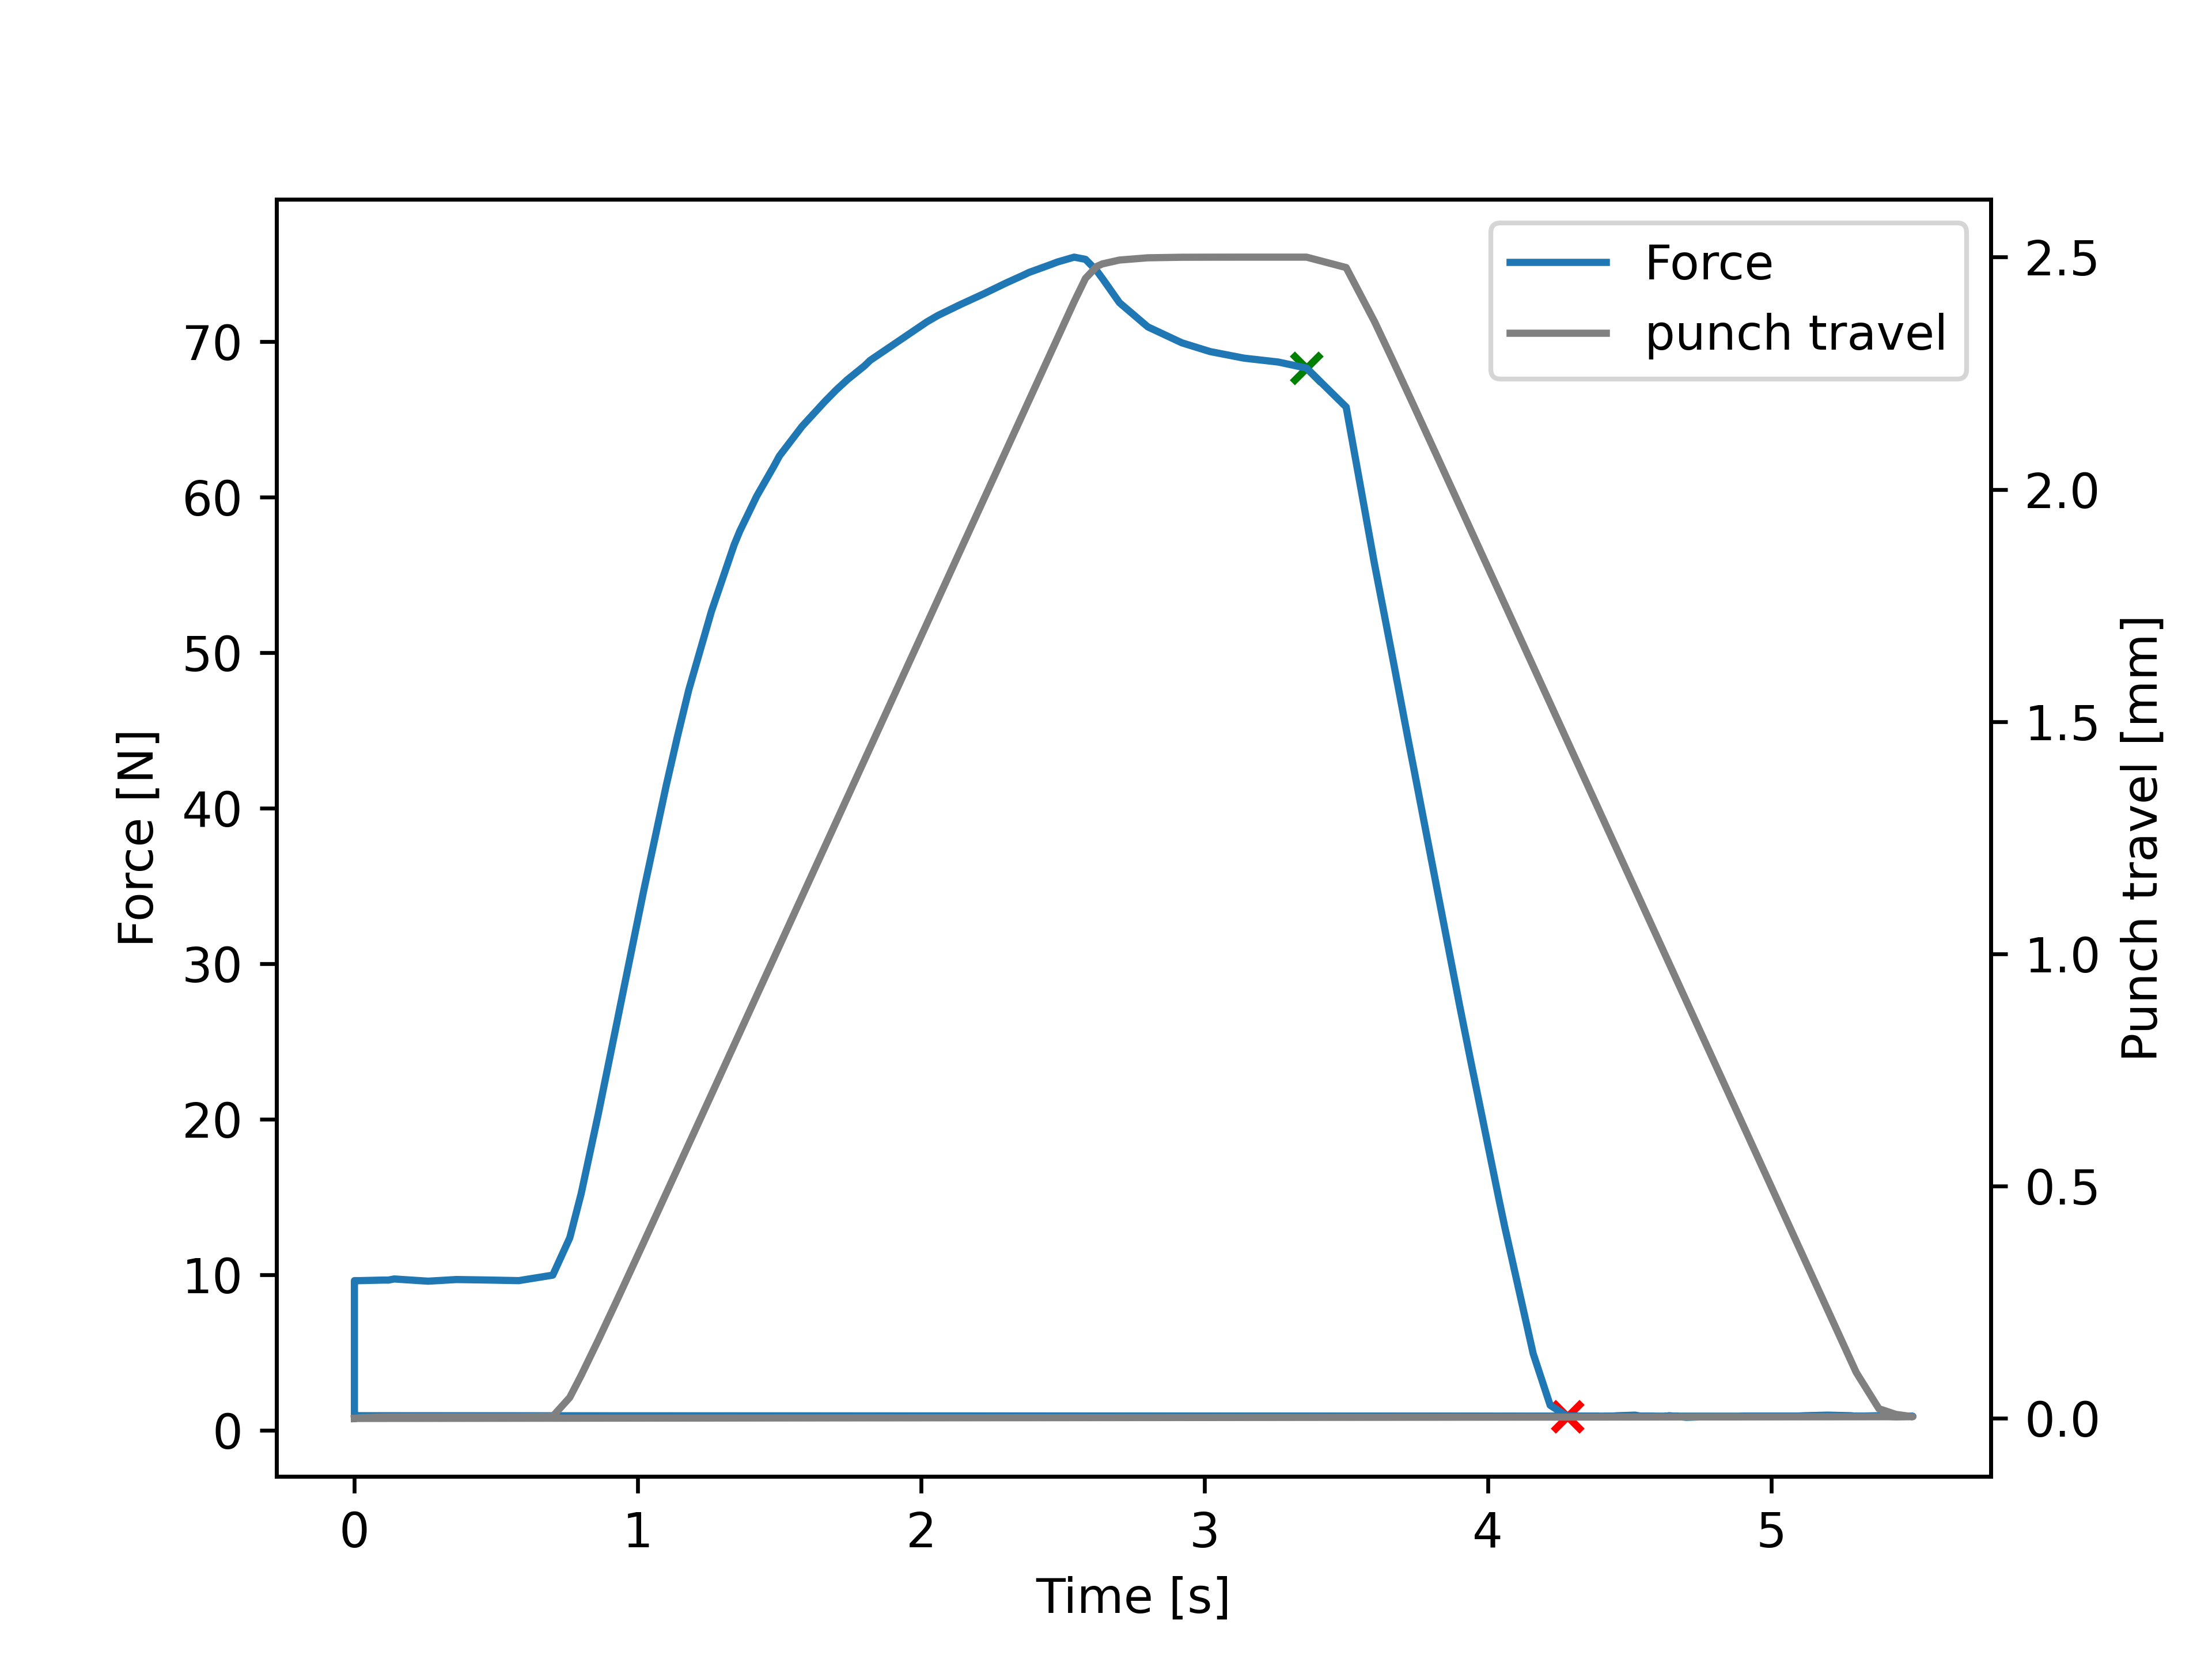
\includegraphics[width=0.7\textwidth]{springback_measured}
    \caption{A steel metal sheet was bent with a punch penetration of 5 mm the spring back is 0.37 mm. The blue line shows the force and the blue line shows the punch penetration.}
    \label{fig:springback_measured}
\end{figure}






% \paragraph{Bend deduction:}
% Measuring the bend deduction is more complex. After a metal sheet is bent, it is hard to measure the flat pattern length because the material is malformed at the bent. 
% As a result, the neutral axis is not in the center of the sheet and hard to measure, but it can be calculated using different approaches. %quelle und ausführlicher und grunlagen teil  
% There are multiple ways to measure the bend deduction described earlier. 
% % K-Faktor Muss noch in theorie teil 
% In this setup, the method described in the DIN6395 was used. This method uses a k-factor which is an approximated value and therefore and therefore it can be inaccurate. (Equation~\ref{eq:kfactor}). % cite DIN norm 

% \begin{equation}\label{eq:kfactor}
%     k=0.65+\frac{1}{2}\log{\frac{r}{s}}
% \end{equation}

% \begin{figure}[ht!] % supposedly places it here ...
% 	\centering
% 	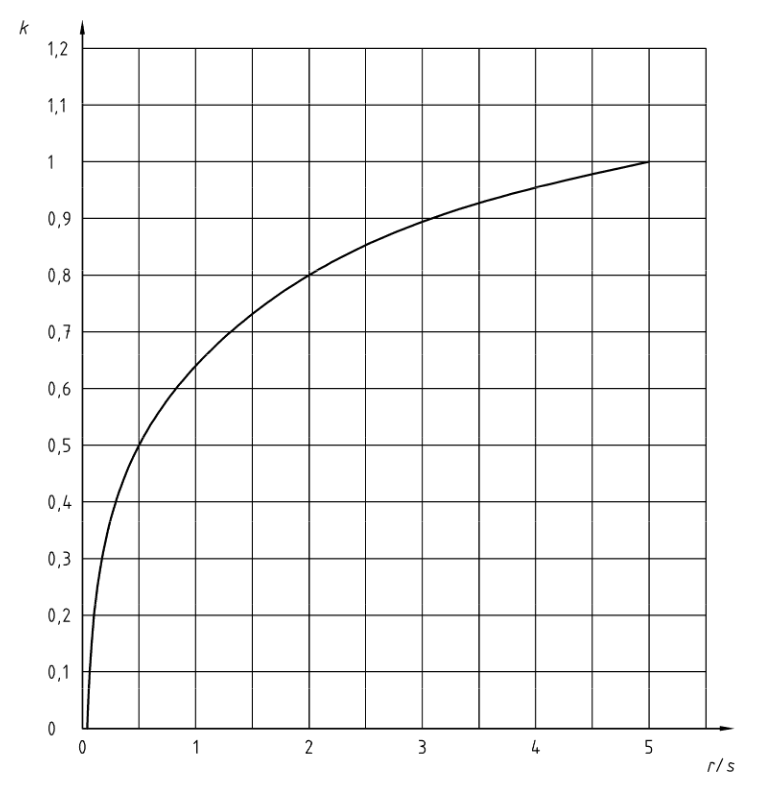
\includegraphics[width=0.5\linewidth]{k-factor}
% 	\caption[Graphical representation of the correction factor]{Graphical representation of the correction factor.}
% 	\label{fig:test1}
% \end{figure}

% The DIN 6935 used the formula for the stretched length, $length=a+b+v$ where \textit{a} and \textit{b} are the side lengths of the sheet and \textit{v} is a correction value for the deduction. \cite{din6935}
% The stretched length is measured different depending on the bending angle.

% \paragraph{Opening angle $\beta 0^\circ$ to $90^\circ$} 
% For opening angles between $0^\circ$and $90^\circ$ the side lengths \textit{a} and \textit{b} are dimensioned from the tangent of the bend to the edge. 
% To calculate the compensation value \textit{v} (Equation~\ref{eq:v1}) is used
% \cite{din6935}.

% \begin{equation}\label{eq:v1}
%         v=\pi*(\frac{180^\circ-}{180^\circ})*(r+\frac{s}{2}*k)-2(r+s)
% \end{equation}

% \begin{figure}[H]
% 	\centering
% 	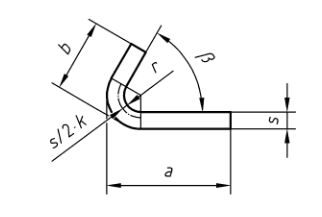
\includegraphics[width=0.5\linewidth]{bending-angle-90}
% 	\caption[Opening angles $\beta 0^\circ$ to $90^\circ$]{Opening angles $\beta 0^\circ$ to $90^\circ$ \cite{din6935}}
% 	\label{fig:v1-image}
% \end{figure}

% \paragraph{Bending angle $\beta90^\circ$ to $165^\circ$} (Equation~\ref{eq:v1})
% For opening angles between $90^\circ$ and $165^\circ$ the side lengths \textit{a} and \textit{b} are dimensioned from the apex to the edge. 
% To calculate the compensation value \textit{v} (Equation~\ref{eq:v1}) is used. 
% \cite{din6935}

% \begin{equation}\label{eq:v2}
%     v=\pi*(\frac{180^\circ-}{180^\circ})*(r+\frac{s}{2}*k)-2(r+s)+\tan{\frac{180^\circ-\beta}{2}}
% \end{equation}

% \begin{figure}[!ht]
% 	\centering
% 	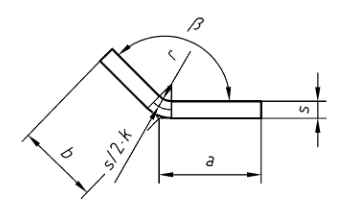
\includegraphics[width=0.5\linewidth]{bending-angle-165}
% 	\caption[Opening angles $\beta90^\circ$ to $165^\circ$]{Opening angles $\beta90^\circ$ to $165^\circ$ \cite{din6935}}
% 	\label{fig:v2-image}
% \end{figure}

% For opening angles between $165^\circ$ and $180^\circ$ the compensation value \textit{v} is 0. The values for v would be negligibly small. \cite{din6935} The side lengths \textit{a} and \textit{b} where measured using the software \textit{ImageJ}. 

% Edge cracking is not measured for now because the steel used has no high-strength and with machine in usage it was not possible to create edge cracking.

% \begin{figure}[!ht]
% 	\centering
% 	\includegraphics[width=0.5\linewidth]{example-image}
% 	\caption[Screenshot ImageJ]{Screenshot ImageJ}
% 	\label{fig:imagej-screenshot}
% \end{figure}


\section{Computational Setup}

\section{Model Selection}

\section{Model Training}








